\chapter{Introdução}
\label{ch:intro}

\section{Descrição do Problema}

\subsection{O Deficiente Visual e as Tecnologias Assistivas}

Um grande desafio atual é promover a inclusão de pessoas com deficiências na sociedade, sejam elas quais forem. Tomando o caso dos deficientes visuais como foco, vários são os desafios enfrentados diariamente, desde a locomoção segura até o processo de aprendizado, ou mesmo o acesso à informação. Como uma forma de amenizar essas dificuldades, garantindo igualdade e promovendo a inclusão social e a cidadania daqueles que possuem alguma deficiência, o Congresso Nacional sancionou algumas leis nesse escopo.

Um exemplo é a Lei 13.146, sancionada em 2015, que instituiu o Estatuto da Pessoa com Deficiência. Em seu texto define acessibilidade em termos de possibilitar, dentre variados direitos, o acesso à informação e a garantia de autonomia para os deficientes. Além disso, trata também de tecnologia assistiva, que pode ser definida, resumidamente, como produtos, serviços ou estratégias que possibilitam ao deficiente a participação em determinada atividade, proporcionando-lhe independência, qualidade de vida e inclusão social \citeC{estatuto}.

Nessa perspectiva, Bersch \citeC{Bersch2013} também define tecnologia assistiva como o conjunto de recursos que amplia as habilidades daqueles que possuem alguma deficiência. Porém, Bersch \citeC{Bersch2013} vai além e assinala o que seria Tecnologia Assistiva em um contexto educacional ou informacional. Em um cenário no qual, antes, a participação ativa do estudante no processo de aprendizagem seria restrita ou praticamente inexistente, a tecnologia assistiva permite que a pessoa com deficiência rompa barreiras que limitam ou impedem o seu acesso à informação ou ao registro dela. Desta forma, favorecendo a participação e a autonomia do estudante em projetos, e por fim, provendo-lhe a manipulação dos objetos de estudo.

Ainda vale reforçar esse conceito, explicitando o ponto de vista sustentado por Radabaugh \citeC{Radabaugh1993} como segue na citação: ``Para as pessoas sem deficiência, a tecnologia torna as coisas mais fáceis. Para as pessoas com deficiência, a tecnologia torna as coisas possíveis.''


No que tange à construção do conhecimento, segundo \citeC{Levy1993}, seu processo está fundamentado principalmente na oralidade e no desenvolvimento da linha de raciocínio durante a escrita do indivíduo. A elaboração do raciocínio, por sua vez, é composta e baseada nas informações acessadas e sentidas pelo sujeito em seu universo. Portanto, no caso do invidente, a informação e a conexão entre os diferentes conceitos aprendidos se dá de forma distinta dos videntes, uma vez que esse processo encontra-se sempre dependente da capacidade do indivíduo de construir significado por meio dos sentidos \citeC{Neto2006}. Sendo assim, é fácil concluir que são pessoas que necessitam de uma abordagem cuidadosa quanto ao consumo de informação.

Um exemplo claro da necessidade de adequação de material didático para uso dos deficientes visuais é o caso do campo de estudos denominado STEM, acrônimo em inglês para Ciências, Tecnologia, Engenharia e Matemática. Os problemas enfrentados pelos deficientes visuais são vários, começando com a dificuldade presente no próprio ambiente de estudo, já que, para que adaptações em infraestrutura sejam feitas, os gastos para a universidade são consideráveis. Consequentemente, esses ajustes necessários para o bom processo de aprendizagem dos deficientes visuais são constantemente negligenciados.

Além disso, muitos professores e colegas não são familiarizados quanto ao proceder em relação aos estudantes invidentes. Porém, provavelmente o problema com maior impacto é a falta de material em si que seja acessível, contendo informações gráficas importantes e que muitas vezes são imprescindíveis ao ensino nessa área. Uma alternativa seria, por exemplo, utilizar técnicas multissensoriais para experimentos científicos, tecnologias com \textit{design} apropriado, como modelos 3D ao invés de figuras em livros, e também softwares que transformam imagens em conteúdo audível \citeC{Beck-Winchatz2008}.

Graças a alguns estudos e projetos que vem sendo desenvolvidos, percebe-se que os deficientes visuais totais ou parciais tem um grande proveito no processo de aprendizagem ao combinar recursos hápticos com instruções ou acompanhamento sonoro. No caso, por exemplo, do sistema apresentado por Plimmer \citeC{Plimmer2008}, os estudantes são ensinados a assinarem o próprio nome por meio de instruções de áudio, enquanto sentem por meio do tato a sua própria assinatura em alto relevo e em tempo real. Desta forma, obteve-se um resultado mais significativo do que o obtido no processo tradicional de ensino, ou seja, sem o auxílio combinatório desses dois recursos.

Além desse trabalho, há também o ensino de desenho à deficientes visuais em cujo processo são empregados sons e diferentes sensações táteis, como diferenças de relevo e textura. O autor enfatiza como esses e outros componentes sensoriais, como por exemplo a temperatura, afetam o deficiente visual, fazendo-o perceber, de maneira indireta, aspectos distintos de um ambiente \citeC{Ballestero-Alvarez2003}.

Vale salientar que as imagens mentais que os invidentes constroem do mundo que os rodeia são semelhantes àquelas criadas pelo indivíduo comum, apesar de serem formadas de maneiras distintas \citeC{Soler1999}. Na ausência de um dos sentidos, a percepção do ambiente e dos objetos vem a partir dos demais sentidos. Por isso, para o deficiente visual, é essencial que variadas estimulações sensoriais estejam conectadas durante o processo de aprendizagem, de forma que possa-se extrair mais informações visuais sobre o objeto de estudo por meio da multissensorialidade \citeC{Ballestero-Alvarez2003}.

Sendo assim, é de suma importância que, para o estudo de determinado objeto, a adaptação da informação visual seja feita de acordo com o sentido mais apropriado para cada caso. Esse conceito é muito bem exemplificado por Ballestero-Alvarez \citeC{Ballestero-Alvarez2003}, quando o autor discute em como a torre \textit{Eiffel} deve ser apresentada a estudantes invidentes em ambientes de estudo. Nesse caso, a opção mais interessante seria, além de disponibilizar-lhes uma maquete, descrever-lhes também a estrutura da torre e seus detalhes, para que assim a experiência de aprendizado seja mais completa, harmonizando os sentidos e proporcionando-lhes uma imagem mental mais completa.

Outro ponto que suporta essa argumentação é que, em muitos casos, a imagem mental formada por videntes não é composta somente por aspectos visuais, mas envolve também outros sentidos de forma simultânea. Logo, o processo de construção do conhecimento de algum objeto para os deficientes visuais, apesar de poder ser em um ritmo distinto do que o é para os videntes, não é, de forma alguma, incompleto ou inferior, podendo ser melhor desenvolvido quando possuem adaptações adequadas para cada caso \citeC{Ballestero-Alvarez2003}.

Portanto, nota-se a importância de plataformas, produtos, serviços ou metodologias que se adequem à realidade do deficiente visual e proporcionem o envolvimento com áreas do conhecimento antes inexploradas por eles ou que os capacitem a exercer funções ou realizar tarefas antes impossíveis. Atualmente, ainda que de forma limitada, há esforços para mudar a realidade de exclusão dos deficientes.

Nesse sentido, podem-se ressaltar alguns trabalhos em desenvolvimento (ou já desenvolvidos) com propósito de acessibilidade. No Museu de Arte da Universidade Federal do Paraná (MusA), foi realizada uma exposição voltada para o público deficiente visual com a transposição de imagens em peças táteis, utilizando materiais para realçar linhas de contorno. Nesse projeto, foram desenvolvidos materiais, em braille e ampliados, de apoio didático sobre as obras de arte e sobre o museu, além de uma sessão de treinamento para os deficientes visuais. Esta sessão é disponível antes da visita, com o objetivo de melhor ambientá-los e possibilitar a formação de uma imagem mental, potencializando assim a experiência durante a exposição \citeC{Fernanda2007}.

Uma plataforma que se destaca é o \textit{DOSVOX}, desenvolvido pela Universidade Federal do Rio de Janeiro \citeC{Borges1998}. O \textit{DOSVOX} consiste em um sistema operacional que possibilita ao deficiente visual o uso do computador para realização de variadas tarefas. Esse sistema se tornou uma ferramenta muito importante para a inclusão dos invidentes, utilizada em todo o Brasil, destacando-se por ser uma ferramenta gratuita. O \textit{DOSVOX} inclui jogos didáticos, tradução do Braille para a escrita latina e vice-versa, leitura de textos por meio de síntese de voz, e a composição e impressão de partituras, entre outras funcionalidades \citeC{Amorim2009}.

Outras tecnologias assistivas que se destacam são o \textit{Jaws} e o \textit{Virtual Vision}, sendo ambos softwares leitores de tela para uso em computador \citeC{Jaws2016} \citeC{VV2016}. Nesse mesmo escopo, existe o software \textit{OpenBook} que escaneia documentos impressos, digitaliza-os e os lê, fornecendo instruções em áudio para o deficiente visual o operar \citeC{OpenBook2016}.
Também foi desenvolvido um dispositivo chamado Linha Braille ou \textit{Display} Braille que, quando conectado ao computador, exibe dinamicamente a informação da tela em braille \citeC{Linha2008}. O dispositivo que possui também botões adicionais para controle dos softwares leitores de tela, unindo a informação sonora à leitura tátil \citeC{Linha2008}. Outra ferramenta interessante é o \textit{TactileView for Tactile Graphics}, que consiste em um software para impressão de figuras e gráficos com pontos em alto relevo \citeC{Tactile2016} \citeC{Amorim2009}.

\subsection{O Deficiente Visual e a Tipografia}

Apesar de toda essa variedade de ferramentas desenvolvidas até hoje, pouco material foi disponibilizado para promover maior aproximação do deficiente visual com a escrita latina e, de forma ainda mais acentuada, com a tipografia. O trabalho que talvez se aproxime mais dessa proposta é o sistema de \citeC{Plimmer2008}, que tem como objetivo ensinar de maneira mais eficaz os deficientes visuais a escrita à mão, começando com a assinatura de seu próprio nome.

%No entanto, seu foco é apenas nos caracteres, na escrita em si, e não na tipografia envolvida.

Um outro exemplo que envolve essa área é o projeto de tipografia ajustável. O sistema possibilita aos deficientes visuais com baixa visão customizar parâmetros da fonte utilizada no documento para melhorar sua legibilidade, de acordo com a necessidade de cada indivíduo \citeC{Arditi2004}. Entretanto, a tipografia é envolvida nesse caso como uma ferramenta para possibilitar a leitura, não sendo o foco do projeto.

%Apesar de o software possibilitar a percepção da diferença causada pela variação dos parâmetros do tipo, o contato com os conceitos da tipografia é nada mais do que empírico e pragmático nesse caso.

A tipografia, assim como a escrita, é utilizada para comunicação. No entanto, assim como em várias formas de arte, a tipografia comunica também por meio de formas, criando uma linguagem visual, estética. Ao associar o significado das palavras à essa linguagem visual, a interpretação é gerada. Se o deficiente visual é privado desse viés visual da informação transmitida por meio da tipografia, ele é também privado de parte da mensagem transmitida, caracterizando uma comunicação que não é bem sucedida em seu todo \citeC{Velasco2015}.

Sensações também podem ser geradas por meio da tipografia. Nesse caso, apesar de o fim principal ser a comunicação, a questão visual e estética pode ser mais importante do que o conteúdo das palavras em si. Este aspecto aproxima a tipografia das artes no sentido de forma de comunicação, conforme é exemplificado na Figura \ref{fig:posterTipo}. Dessa maneira, o deficiente visual é ainda mais prejudicado quando privado dos detalhes da área, já que grande parte da mensagem não se encontra no sentido das palavras ali escritas.


%Nesse sentido, o deficiente visual também é bastante prejudicado quando não tem contato com todo esse universo de logotipos, marcas, filmes, bandas, entre outros campos no quais é aplicada a tipografia e nos quais os videntes estão imersos .
Por gerar sensações distintas, uma das aplicações mais importantes da tipografia é diferenciar estilos, produtos e marcas. A tipografia desempenha papel importante no cenário atual, presente em boa parte dos artigos do cotidiano. A cultura popular, por exemplo, se vale da tipografia em conteúdos como filmes, séries, propagandas comerciais, capas de álbuns musicais, cartazes diversos, marcas de empresas, mídias sociais, entre outros. Portanto, uma miríade de contextos culturais e de informação com qual o deficiente visual não tem contato, contribuindo para a sua exclusão\citeC{Velasco2015}.

Além disso, a tipografia também tem relevância no campo histórico, no qual influencia e pelo qual é influenciada. Um exemplo é o evento da invenção da imprensa. Antes de sua criação, a comunicação e o acesso à informação eram exclusivistas pois, apenas poucas pessoas sabiam escrever e tinham acesso a esse tipo de material como, por exemplo, os monges. Porém, com o advento da imprensa e, consequentemente, da tipografia, houve um crescimento exponencial da comunicação e da distribuição do conhecimento por meio da escrita, inclusive a Reforma Protestante valeu-se da imprensa para disseminação de seus ideais \citeC{Costa2008}. Por esse aspecto, a tipografia foi essencial para a propagação do conhecimento.

\begin{figure}[H]
 \centering
  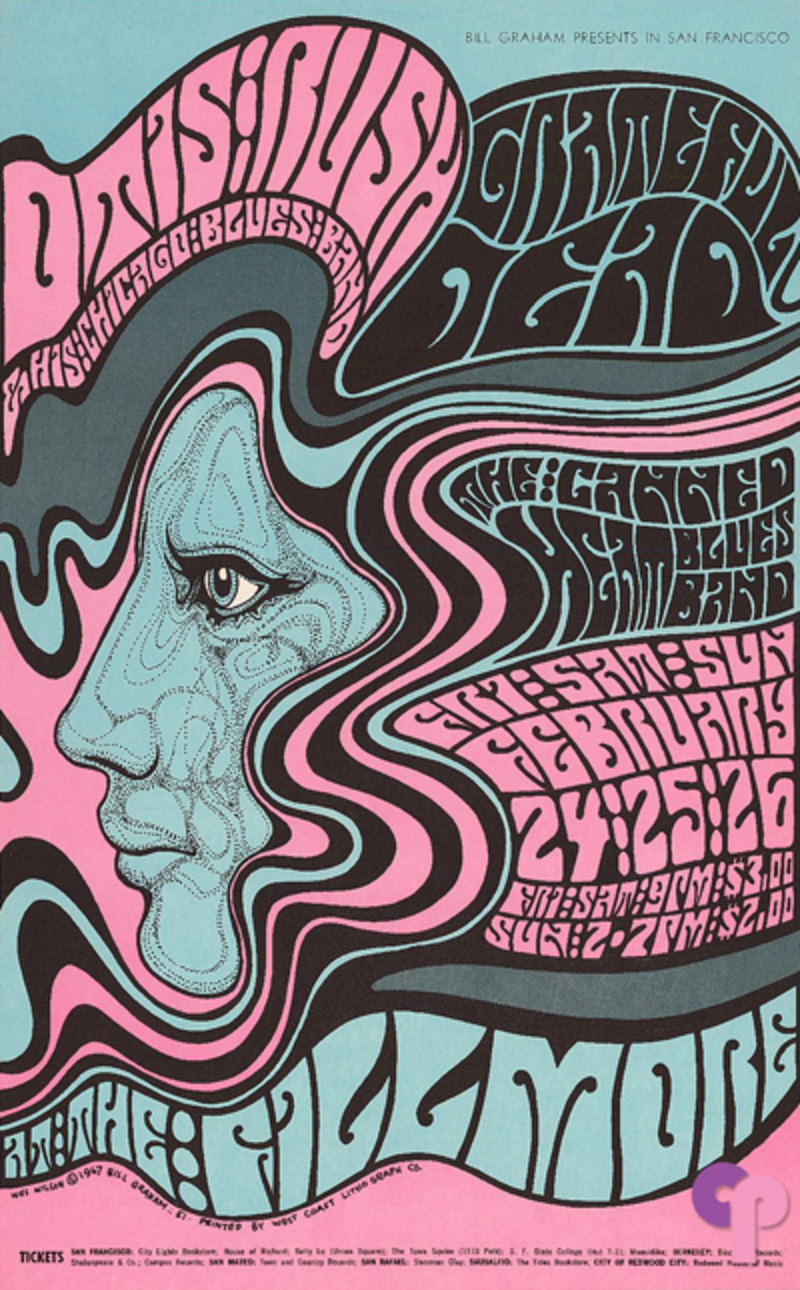
\includegraphics[width=0.4\linewidth]{figuras/posterTipo.pdf}
  \caption{Exemplo de tipografia aplicada como comunicação majoritariamente estética. Cartaz de Bill Graham feito para banda de \textit{Blues} de Chicago \citeC{graham2017}.}
  \label{fig:posterTipo}
\end{figure}


A tipografia também sofreu influências e foi moldada, tanto por limitações físicas como por correntes filosóficas adotadas pela sociedade. As limitações consistem no processo de fabricação dos tipos: metal, madeira, fotocomposição ou digital, sendo que cada um desses processos possui suas características próprias.


\section{Proposta de Projeto}

Tendo em vista que o deficiente visual possui pouco contato com a área, propõe-se um sistema auxiliar ao ensino de tipografia para deficientes visuais. Abre-se, então, a oportunidade de um novo tipo de leitura. Para o deficiente visual, abre-se um novo horizonte de conhecimento e interação dos invidentes com os caracteres latinos, usados em mais de um terço do mundo \citeC{World2015}. Ainda, a mitigação da exclusão cultural do deficiente visual, que é agravada pelo distanciamento desse grupo em relação ao elemento estético da tipografia.

Os deficientes visuais se encontravam em um ``gueto cultural'' antes do desenvolvimento de ferramentas como o \textit{DOSVOX} que possibilitassem a tradução dos textos escritos em braille para os caracteres latinos. Suas produções ficavam restritas já que raros videntes sabem ler ou escrever em braille e o acesso à informação ficava comprometido \citeC{Borges1998}. Nesse sentido, o projeto aqui proposto contribui também para a eliminação deste ``gueto cultural''.

Como já enfatizado, Neto \citeC{Neto2006} faz um trabalho voltado para responder a questão sobre qual é a influência que o uso das tecnologias assistivas de informação e comunicação tem sobre a experiência do deficiente visual com a escrita e com a leitura por meio do braille. Por outro lado, a proposta aqui apresentada estende esse objetivo ao tentar inserir o deficiente visual em um contexto que diz respeito, não somente aos caracteres utilizados pela língua nativa do país onde vive, mas também ensinar aspectos a respeito à anatomia de cada letra, permitindo diferenciar os caracteres entre si e os seus estilos, aproximando-o da experiência que um vidente tem ao ler qualquer mídia.

O sistema proposto possui não só um caráter de aproximação do invidente com a escrita e com os diversos estilos tipográficos, proporciona-lhe também a opção de se aprofundar nos estudos da tipografia, incluindo conceitos, aplicações e contextos históricos. Sendo assim, esse projeto apresenta um material inédito, por ser uma tecnologia assistiva que proporciona ao invidente o contato com uma informação antes restrita a ele, apesar de inicialmente ainda ser uma tecnologia com opções limitadas.

Além do mais, como o envolvimento dos deficientes visuais com o mundo digital da informática está crescendo, há necessidade de cursos formativos para que o invidente possa conhecer melhor as possibilidades de leitura e escrita utilizando as tecnologias assistivas desse natureza \citeC{Neto2006}. Sendo assim, um maior contato do deficiente com a tipografia é um fator predominante nesse contexto e que deve ser ensinado ao deficiente visual, sendo uma área ainda pouco explorada.

A proposta para esse projeto foi idealizada primeiramente por uma estudante de \textit{Design} da Universidade de Brasília, com a qual esse projeto foi desenvolvido em parceria. O projeto consiste em um sistema auxiliar para ensino de tipografia a deficientes visuais \citeC{Cruz2016}. O sistema, denominado Tipo Tátil, trata-se de um material tátil, com a qual o deficiente visual pode interagir e um material escrito, que traz as informações necessárias para auxiliar o ensino dessa área.

A parte tátil do sistema consiste de placas tridimensionais com as letras inseridas em alto relevo e réplicas avulsas, como ilustrado na Figura \ref{fig:placas}. Como prospota inicial, escolheram-se nove tipografias para compor o projeto, escolha baseada em uma classificação tipográfica específica (ver Capítulo \ref{ch:Tipografia}). Na Figura \ref{fig:tipografias}, apresentam-se as nove tipografias listadas, exemplificadas pelo caractere ``a'' como exemplo.

\begin{figure}[H]
 \centering
  \includegraphics[width=0.75\linewidth]{figuras/placasA.pdf}
  \caption{Conjunto de placas apresentando as nove tipografias \citeC{cruz2017}}
  \label{fig:placas}
\end{figure}

Esse sistema provê ao deficiente visual a diferenciação das características anatômicas e estilísticas de variados tipos, contando com o alfabeto completo para cada tipografia e também com um sistema pedagógico (material escrito) para que os deficientes visuais possam compreender as nuances e sutilezas da variedade de fontes tipográficas da escrita latina, entendendo seus significados formais e históricos \citeC{Cruz2016} \citeC{cruz2017}. Além disso, o projeto foi expandido para abarcar um exemplo de escrita cursiva, também apresentando placas com letras em alto relevo, bem como caracteres especiais de acentuação e operações matemáticas.

\begin{figure}[H]
 \centering
  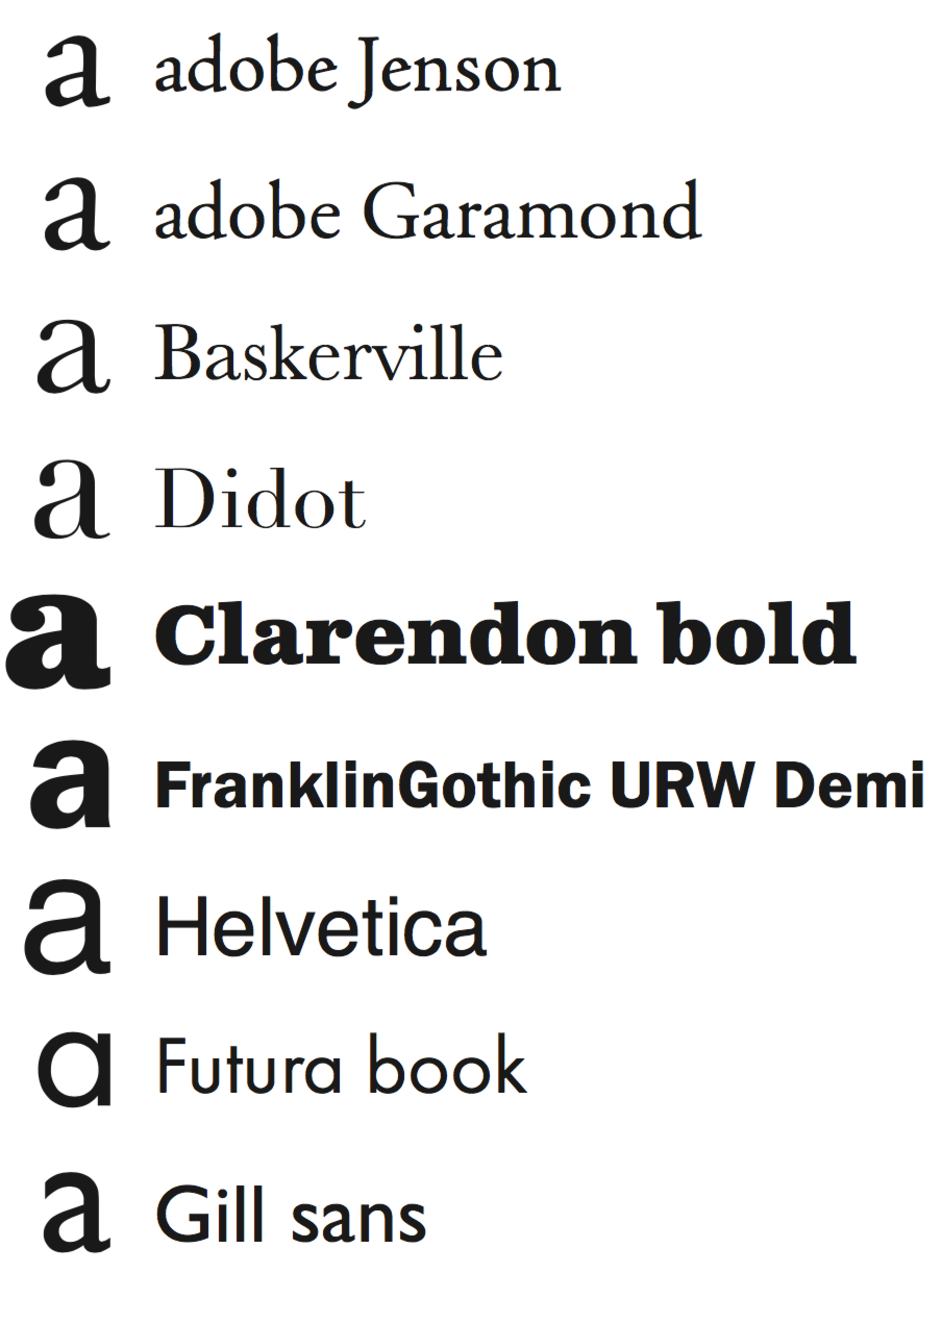
\includegraphics[width=0.4\linewidth]{figuras/tipografias.pdf}
  \caption{Tipografias que compõem o projeto.}
  \label{fig:tipografias}
\end{figure}


%Além disso,
De modo a tornar o projeto ainda mais completo, com o intuito de proporcionar ao deficiente a autonomia para estudar, de acordo com o conceito da tecnologia assistiva, e sabendo que maior eficácia é alcançada quando proporcionados estímulos multissensoriais, propõe-se a implementação de um sistema computacional auxiliar e interativo para guiar o deficiente visual durante o uso do produto de tecnologia assistiva \citeC{Ballestero-Alvarez2003}.

O sistema funcionaria com o usuário inserindo, em uma área pré-determinada, a peça sobre a qual deseja maiores informações. Então, a partir de captura de imagem (propõe-se uma \textit{webcam}) ocorreria o reconhecimento da tipografia e do caractere da peça e, por meio da síntese de voz, seriam providas ao usuário informações detalhadas sobre os conceitos acerca daquela tipografia, a saber, aplicações, especificações estilísticas e contexto histórico, conduzindo-o durante o processo de interação com a peça.

O escopo deste documento é o desenvolvimento e resultado da parte central do sistema: o algoritmo de reconhecimento de padrões que é utilizado para a classificação da tipografia da peça (tipo) contida em uma imagem de entrada (Figura \ref{fig:placas}).

Para o reconhecimento de padrões, serão empregadas técnicas de aprendizado de máquina (\textit{Machine Learning}). Geralmente essa é a melhor abordagem para se tratar problemas de reconhecimento de padrões, apesar de também haver a possibilidade de serem aplicadas outras técnicas como as heurísticas \citeC{Bishop2006}. Aprendizado de máquina é uma técnica pertencente ao campo da Inteligência Artificial e tem como objetivo obter sistemas capazes de aprender de forma automática, sem terem sido explicitamente programados \citeC{samuel1959} \citeC{ng2016}. O processo de aprendizado do sistema ocorre por meio de experiências e de soluções bem-sucedidas de casos anteriores \citeC{libralao2003}. As técnicas de aprendizado de máquina são aplicadas em problemas para extrair conceitos a partir de um banco de dados (reconhendo padrões). Sendo assim, a constituição do banco de dados (suficientemente grande) é uma parte importante do projeto e irá compor o conjunto de treinamento para o algoritmo de aprendizado de máquina.

O banco de dados, neste projeto, é formado por imagens contendo os diversos tipos. Sendo assim, as categorias das imagens são previamente conhecidas e rotuladas, sendo elas o nome de cada tipografia. Desta forma, o processo de aprendizado de máquina é denominado um problema de aprendizado supervisionado (\textit{supervised learning}).

Porém, em muitas aplicações, devido à grande variação dos dados de entrada, o algoritmo compreende apenas uma pequena porção de todo o conjunto que deseja-se classificar. Sendo assim, uma prática comum é passar os dados (neste caso, as imagens) por um método de pré-processamento, de forma a uniformizar as imagens de entrada. Um exemplo do processo adotado em um algoritmo de reconhecimento óptico de caracteres (OCR, \textit{Optical Character Recognition}, em inglês) é apresentado na Figura \ref{fig:etapas}. Está é uma abordagem comum para a solução desse tipo de problema, sendo um caso semelhante ao aqui proposto \citeC{Bishop2006} \citeC{Miranda2013}.

Os classificadores empregados neste projeto são a Máquina de Vetor de Suporte (SVM, em inglês \textit{Support Vector Machine}) e a Floresta Aleatória (\textit{Random Forest Classifier}). Máquina de Vetor de Suporte é um modelo classificador paramétrico, baseado na Teoria de Aprendizado Estatístico, podendo ser usada em casos de classificação ou regressão linear \citeC{lorena2007}. Já a Floresta Aleatória é uma extensão do modelo de Árvores de Regressão e de Classificação e sua predição baseia-se em dividir recursivamente o conjunto de dados, com base nos valores de preditores \citeC{maindonald2007}.

\begin{figure}[H]
  \centering
  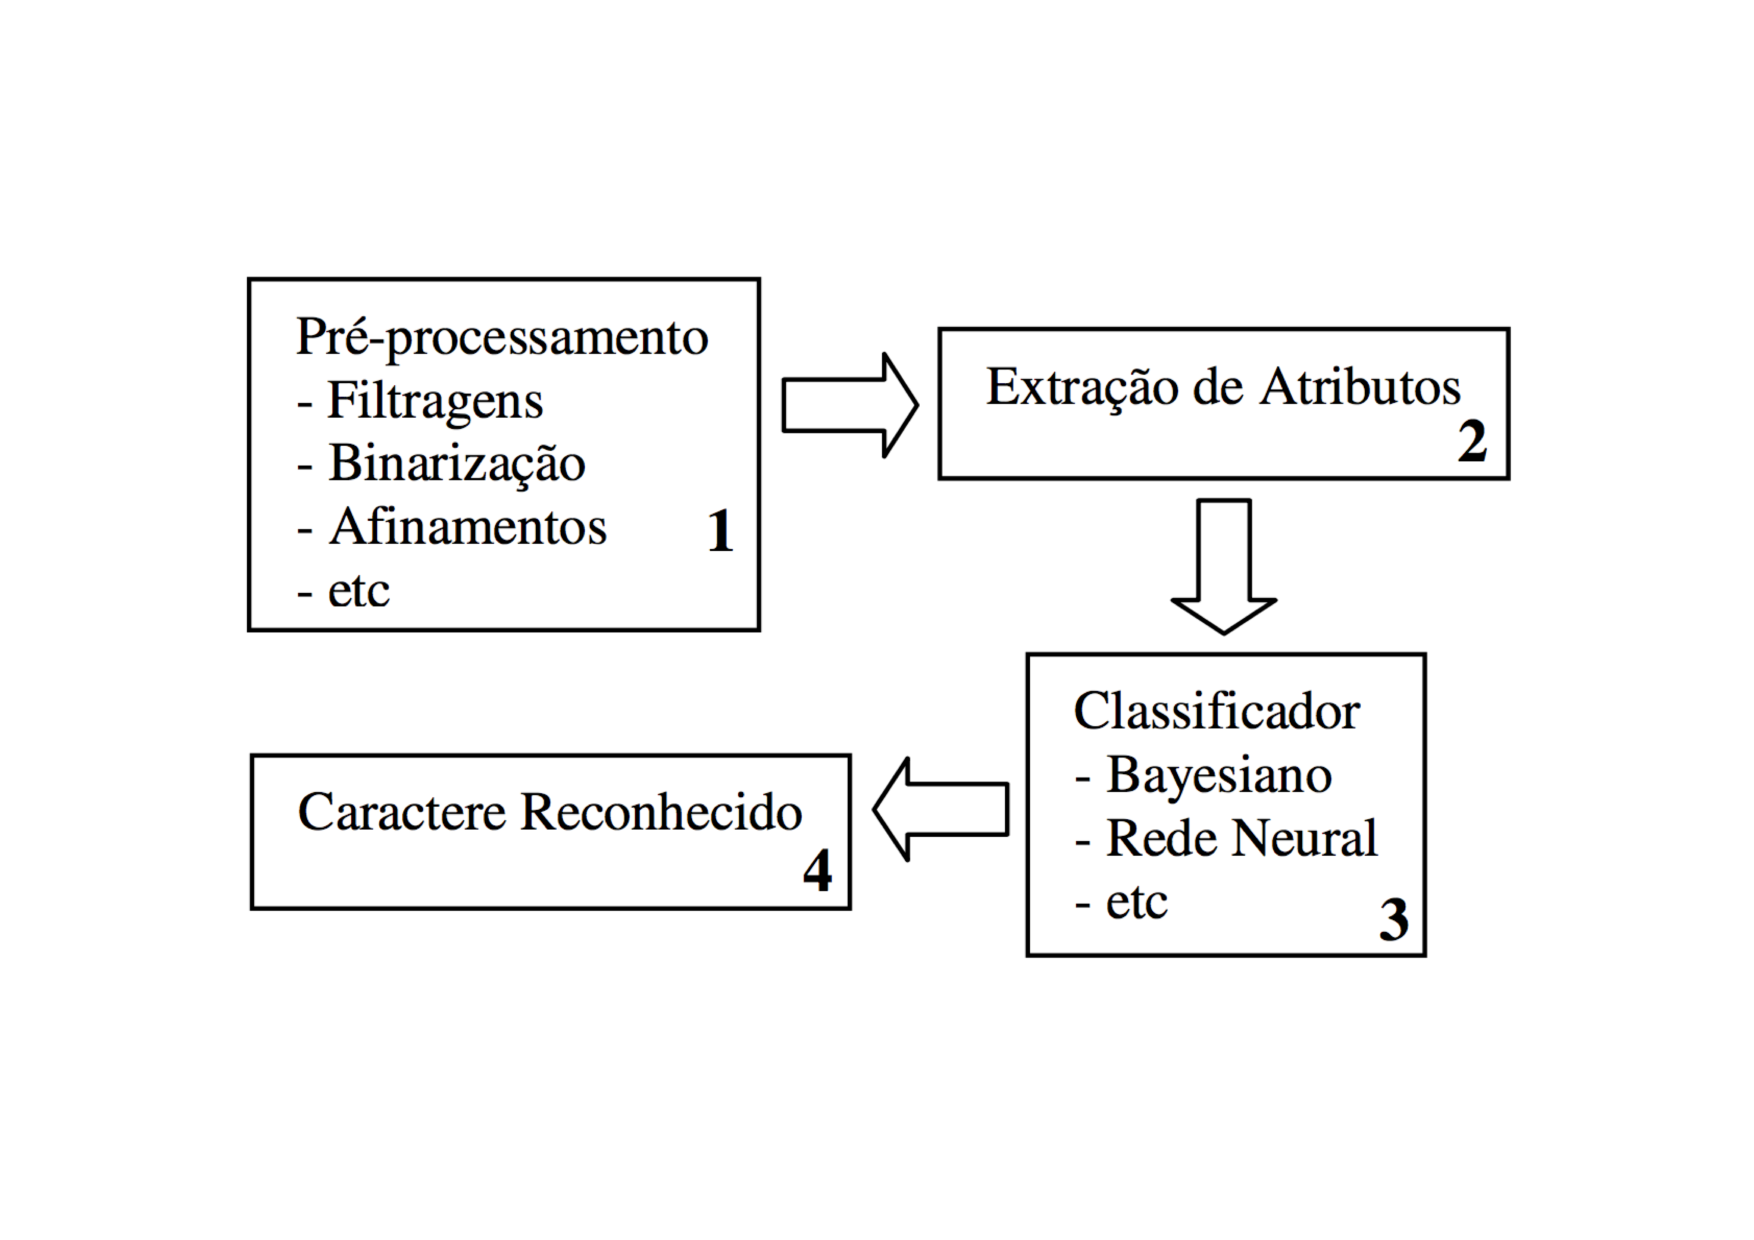
\includegraphics[width=0.7\linewidth]{figuras/etapaProcessamento.pdf}
  \caption{Etapas do Processo de Reconhecimento de Caracteres \citeC{miranda2013handwritten}}
  \label{fig:etapas}
\end{figure}

Vários dos softwares de tecnologia assitiva utilizam OCR em sua composição para leitura de tela ou de arquivos. Entre os exemplos, podem-se citar o \textit{OpenBook}, o \textit{Jaws} e o \textit{Virtual Vision} \citeC{OpenBook2016} \citeC{Jaws2016} \citeC{VV2016}. No sistema de auxílio ao ensino da escrita à mão para deficientes visuais proposto por Plimmer \citeC{Plimmer2008}, também utiliza-se OCR e uma abordagem semelhante à de Miranda \citeC{Miranda2013}. Desta forma, percebe-se que esse campo de reconhecimento de caracteres favorece o desenvolvimento de várias tecnologias assistivas.

Apesar de o reconhecimento de padrões ter raízes históricas na ciência, a sua abordagem com aprendizado de máquina encontra-se em um momento ímpar de crescimento. Graças ao veloz crescimento e popularização dos dispositivos com câmera, como smartphones e tablets, e também da internet e redes sociais, o volume de imagens e vídeos compartilhados na rede é imenso. Além disso, a capacidade de processamento dos computadores também apresenta um crescimento acelerado. Dessa forma, o aprendizado de máquina enfrenta um ótimo momento  para seu desenvolvimento, já que está acessível um grande banco de dados de imagens para compor o conjunto de treinamento e o hardware necessário para o processamento também \citeC{Feris2016}. Sendo assim, várias são as aplicações nessa área, desde utilidades no campo das ciências sociais até o campo da criminalística \citeC{Grimmer2015} \citeC{li2015clothing}. Para o reconhecimento de padrões na área de Visão Comuputacional, o aprendizado de máquina é muito importante, sendo aplicado em várias situações como, por exemplo, na localização de prédios, no reconhecimento facial e na edição inteligente de fotos \citeC{szeliski2010computer}.

Por outro lado, o reconhecimento de tipos (OFR, \textit{Optical Font Recognition}, em inglês) continua como um campo que não é muito explorado pela comunidade de pesquisadores \citeC{Zramdini1995}. Geralmente, quando o problema é atacado, utiliza-se o reconhecimento de tipos apenas como forma de melhoria para o reconhecimento de caracteres, especialmente quando um documento possui variadas tipografias, ou ainda para uma possível classificação de documentos, que podem ser diferenciados de acordo com a tipografia ali empregada \citeC{Shi1997} \citeC{Manna1999}. Outra situação na qual o reconhecimento de fontes é utilizado é no reconhecimento de caracteres não-latinos, como chineses, arábicos ou farsi \citeC{Yang2006} \citeC{Slimane2013} \citeC{Zahedi2011}.

Nesse contexto, o trabalho de Zramdini \citeC{Zramdini1995} tem como diferencial um sistema que considera todas as variedades anatômicas e intrafamiliares das fontes e por também propor uma combinação entre o reconhecimento de fontes e de caracteres, o que faz parte do objetivo do sistema final proposto para o projeto apresentado neste documento. No entanto, Zramdini \citeC{Zramdini1995} apresenta uma abordagem distinta da aplicada nesse projeto para o reconhecimento das tipografias. Em seu trabalho, o autor utiliza as características dos caracteres, baseadas em propriedades locais das letras individuais, tais como a anatomia de cada letra e as peculiaridades de determinadas tipografias. Por exemplo, uma das características utilizadas é o estilo de serifa, para estimá-lo, computa-se a borda de cada caractere e analisa-se o comprimento da borda, para determinar o estilo da serifa. Uma das restrições deste trabalho \citeC{Zramdini1995} é que, para que possa ocorrer a classificação de tipografia baseada em comparações estruturais entre os tipos, deve-se ter um conhecimento prévio em relação à qual classe o caractere avaliado pertence. Sendo asim, o autor desenvolveu um sistema classificador distinto para cada caractere. Este sistema primeiramente aplica um algoritmo de OCR para identificar o caractere e, posteriormente, o modelo classificador para classificar a tipografia (OFR).

Já no caso do projeto apresentado neste trabalho, os caracteres foram tratados simplesmente como imagens, não sendo um requisito o conhecimento prévio em relação à qual carecetere se trata. Os seus atributos foram extraídos, também de forma local, por meio do Padrão Binário Local (LBP, \textit{Local Binary Pattern} em inglês), um operador proposto em 1994 e utilizado em visão computacional, especialmente em classificação de texturas e reconhecimento de faces \citeC{ojala1994} \citeC{do2012}.

\section{Estrutura do Trabalho}

Este documento divide-se de forma a apresentar uma estrutura que facilite o entendimento do leitor em relação ao desenvolvimento do sistema de reconhecimento de padrões em tipos para classificação das tipografias presentes no projeto explicitado na seção anterior. No Capítulo \ref{ch:Tipografia}, apresentam-se conceitos básicos de tipografia, relevantes para o projeto. No Capítulo \ref{ch:ML} são explicados os fundamentos teóricos dos modelos de extração de atributos e de classificação, bem como a estrutura do algoritmo de Aprendizado de Máquina.

Já nos Capítulos seguintes, a saber, \ref{ch:Metodologia} e \ref{ch:Resultados}, é detalhado o desenvolvimento do trabalho especificamente, com todos os algoritmos implementados na metodologia e os resultados alcançados, bem como sua análise. No Capítulo \ref{ch:Conclusao}, apresentam-se as conclusões e discutem-se quais os objetivos do projeto já foram alcançados e quais serão os passos futuros.


%\begin{figure}[H]
%  \centering
%  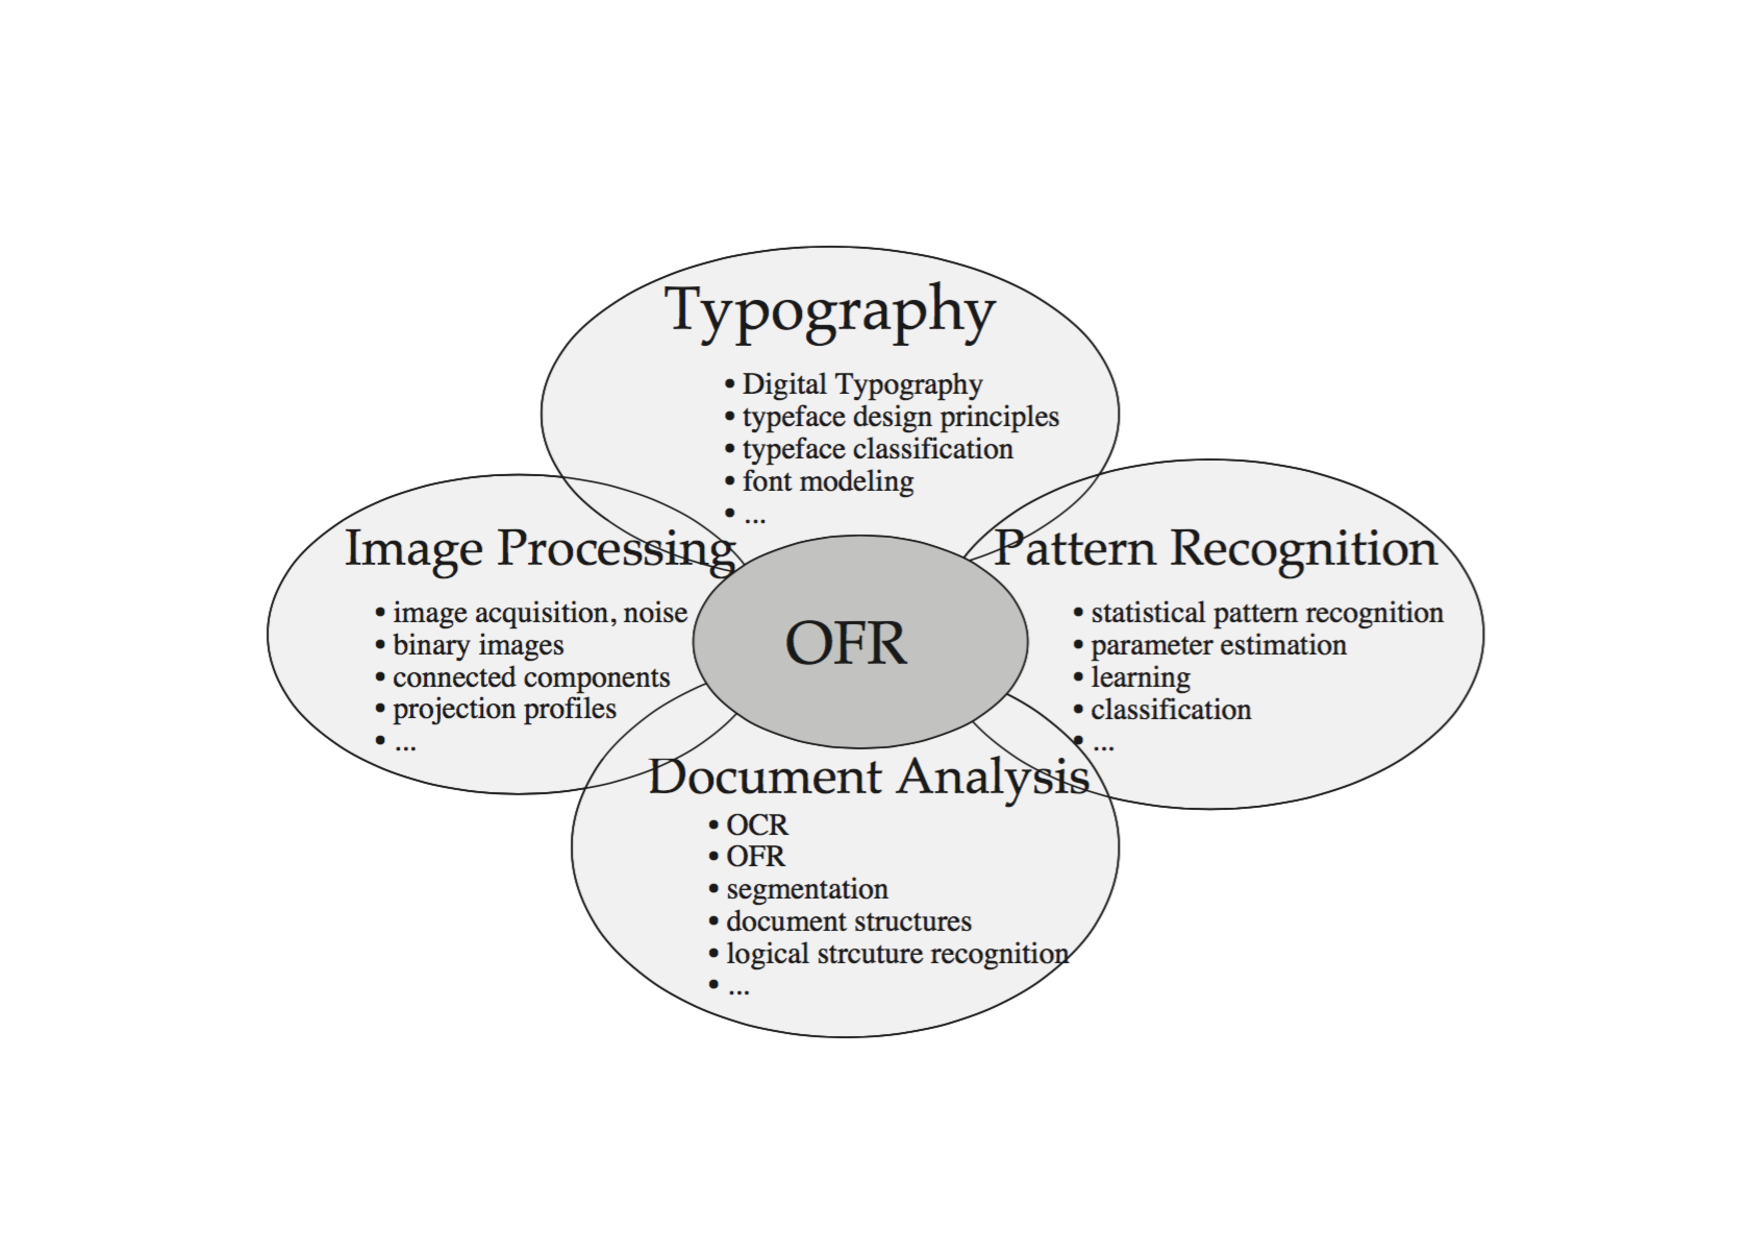
\includegraphics[width=0.8\linewidth]{figuras/OFRareas.pdf}
%  \caption{Áreas Necessárias para Reconhecimento de Fontes - \textbf{Fonte:} \citeC{Zramdini1995}}
%  \label{fig:OFRareas}
%\end{figure}



%for the recognition of characters, but the rec- ognitionofthetypeoffontsisdisregarded \citeC{aviles2005}
%The methodology applied in our processing im- age algorithm was based on to estimate features not over full image, instead of this, feature estima- tionwasdoneoverregionsofimagescalled‘‘sub- image’’.Theestimatedattributearraysofeach sub-image were the reference database to recognize thetypeofeachfont(100windowsaretakenran- domlyovereachfulltext) \citeC{aviles2005}



%Uma citação~\cite{artigo:2015}.

%As citações são feitas usando o comando~\texttt{\textbackslash cite}. Para usar colchetes nas citações, use o comando~\texttt{\textbackslash citeC}. Exemplo \citeC{artigo:2015}.


%blá blá, blá \cite{artigo:2015}
